% This work is licensed under the Creative Commons
% Attribution-NonCommercial-ShareAlike 4.0 International License. To view a copy
% of this license, visit http://creativecommons.org/licenses/by-nc-sa/4.0/ or
% send a letter to Creative Commons, PO Box 1866, Mountain View, CA 94042, USA.

Empfohlene Literatur
\begin{itemize}
	\item Ciarlet: the finite element method for elliptical problems (1987/2002)
	\item Brenner, Scott: the mathmatical theory of finite element method (2002)
	\item Schmidt, Siebert: design of adaptive finite element software
\end{itemize}

\section{Beispiele und Motivation}

\begin{align*}
	\laplace u &= f \quad  \text{in }  \Omega\\
		  	 u &= 0 \quad \text{auf } \partial\Omega
\end{align*}

$\rightarrow$ \underline{finite Differenzen}\nl
z.B. $\Omega = (0,1) \times (0,1)$ mit der Notation
\begin{align*}
	 u&= u(x,y)				 &   u_{ij}&\ \text{approximiert}\ u(x_i,y_j)\\
	(x_i, y_j) &\in \Omega, \quad i,j = 1,\dots,N&  h&= x_{i+1} - x_i = y_{i+1}-y_i
\end{align*}

-Taylorentwicklung
\begin{align*}
	u(x_{i+1},y_j) &= 	u(x_{i},y_j) + 	h\partial_x u(x_{i},y_j) + \frac{1}{2}h^2 \partial_{xx}	u(x_i,y_j) + \bigo(h^3)\\
	u(x_{i-1},y_j) &= 	u(x_{i},y_j) - 	h\partial_x u(x_{i},y_j) + \frac{1}{2}h^2 \partial_{xx}	u(x_i,y_j) + \bigo(h^3)\\
\end{align*}
$\implies$
\begin{align*}
	\partial_{xx} u(x_i,y_j) &= \frac{1}{h^2}\big(	u(x_{i+1},y_j) - 2u(x_i,y_j) + 	u(x_{i-1},y_j) \big) + \bigo(h)\\
	\partial_{yy} u(x_i,y_j) &= \frac{1}{h^2}\big(	u(x_i,y_{j+1}) - 2u(x_i,y_j) + 	u(x_i,y_{j-1}) \big) + \bigo(h)
\end{align*}

\begin{equation*}
	\laplace u(x_i,y_j) = \frac{1}{h^2} \left( u_{i+1 j} + u_{i-1 j} + u_{i j+1} + u_{i j-1} - 4u_{i j} \right)
\end{equation*}

$\implies$
\begin{align*}
	 u_{i+1 j} + u_{i-1 j} + u_{i j+1} + u_{i j-1} - 4u_{i j} &= f_{i j}h^2 & & (x_i,y_j) \in \Omega\\
	 u_{i j} &= 0 & & (x_i,y_j) \in \partial\Omega 
\end{align*}

Benenne die $u_{ij}$ in $u_k$ um, mit $k = iN+j$. Bezeichne nun $U_k = u_{ij}$ und $F_k = f_{ij} $.

$\implies$
\begin{equation*}
	AU = F 
\end{equation*}
mit 
\begin{align*}
	A = \frac{1}{h^2}
	\begin{pmatrix}
	A_0       & I        & 0		&\dots  & 0     \\
	I		  & A_0 	 & I 		&\ddots & \vdots\\
	0		  & I        & \ddots 	&		& 0     \\
	\vdots    & \ddots   & 		  	& A_0	&	I   \\
	0		  & \dots 	 & 0  		& I 	& A_0   \\
	\end{pmatrix}, 
	\quad
	A_0 = 
	\begin{pmatrix}
	-4    		& 1      & 		  & \textbf{0}  \\
	1	  		& -4 	 & \ddots & 			\\
		  		& \ddots & \ddots &	1   \\
	\textbf{0}	& 	     & 1 	  & -4   \\
	\end{pmatrix}
\end{align*}

%% maybe Vor- und Nachteile

$\rightarrow$ \underline{finite Elemente}
\begin{align*}
  \laplace u &= f \quad  \text{in}\  \Omega\\
  u &= 0 \quad \text{auf}\ \partial\Omega
\end{align*}

\begin{equation*}
	\int_\Omega (\laplace u) v \diff x = \int_\Omega fv \diff x \text { f\"ur } v\in C^1(\overline{\Omega}), \; v=0 \text{ auf } \partial \Omega
\end{equation*}

\begin{align*}
	\int_\Omega \text{div}( \nabla u) v \diff x
	&= \int_\Omega \text{div}( v \nabla u ) \diff x -	\int_\Omega \nabla u \cdot \nabla v \diff x \\
	&=  \underbrace{\int_{\partial\Omega}  v \nabla u  \cdot \vartheta \diff x}_{=0\text{ s. Def. v}} -	\int_\Omega \nabla u \cdot \nabla v \diff x \\
	&=  \int_\Omega fv \diff x
\end{align*}

Dies gilt für $u \in X$ s.d. $\forall v\in X$ f\"ur einen passenden Funktionenraum $X$.
Diese Form wird schwache Formulierung oder Variationsformulierung und nur erste Ableitungen werden benötigt.
\\
Gesucht wird eine Approximation $u_h$ in endlich dimensionalen Raum $X_h$ s.d. $X_h \to X$ f\"ur $h \to 0$.\enter
$u_h$ erf\"ullt f\"ur alle $v\in X_h$ die Gleichung
\begin{equation*}
	-	\int_\Omega \nabla u_h \cdot \nabla v_h \diff x = \int_\Omega fv_h \diff x.
\end{equation*}

Sei $\varphi_1,\dots, \varphi_n$ eine Basis von $X_h$, dann gilt:
\begin{equation*}
	u_h = \displaystyle\sum_{i=1}^N u_i\varphi_i 
\end{equation*}
und mit $v=\varphi_j$ folgt 
\begin{equation*}
	- \displaystyle\sum_{i=1}^N u_i \int_\Omega \nabla \varphi_i \cdot \nabla \varphi_j \diff x = \int_\Omega f\varphi_j \diff x \qquad j=1,\dots,N
\end{equation*}
mit 
\begin{align*}
	A_{ij} = \int_\Omega \nabla \varphi_i \cdot \nabla \varphi_j \diff x, \quad \quad F_j = \int_\Omega f \varphi_j \diff x
\end{align*}
$\implies$
\begin{align*}
	- \displaystyle\sum_{i=1}^N A_{ij}u_i &= F_{ij}\\
	AU &=F\\
	\text{mit } U &=
	\begin{pmatrix}
	u_1      \\
	\vdots	 \\
	u_n	  	 \\
	\end{pmatrix}
\end{align*} 

W\"ahle nun die Testfunktionen $\varphi_j$ mit kleinem Tr\"ager so, dass $A$ dünnbesetzt ist.
\begin{equation*}
	\text{spt}(\varphi_j) = \overline{\Big\{  x \in \Omega: \varphi_j(x) \neq 0 \Big\}}
\end{equation*}

%  Obige schreibweise gefällt mir nicht

Definiere $\varphi_j(b_i) = \delta_{ij}$ und $\varphi_j$ linear in allen Teilabschnitten $\tau \in T$, wobei $T$ eine Triangulierung ist und 
\begin{equation*}
	\overline{\Omega} = \bigcup\limits_{\tau\in T}\tau
\end{equation*}
gilt.


\begin{figure}[h!]
	\center

	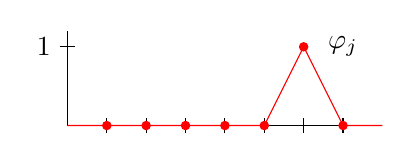
\begin{tikzpicture}[scale=1]
	%\fill[black!20!white] (2.15,0) -- ++(0,0.35) -- ++(0.65,0.26) -- ++(0,-0.61) -- cycle;
	%\draw (2.15,0) 
	\draw (0,0) -- ++(0,1.2);
	\draw (0,0) -- ++(4,0);

	\draw[red] (0,0) -- ++(2.5,0) -- ++(0.5,1) -- ++(0.5,-1) -- ++(0.5,0);
	%\filldraw (2.15,0.35) circle (0.4pt);
	
	\draw (-0.1,1) -- ++(0.2,0);
	
	\draw (0.5,-0.1) -- ++(0,0.2);
	\draw (1  ,-0.1) -- ++(0,0.2);
	\draw (1.5,-0.1) -- ++(0,0.2);
	\draw (2  ,-0.1) -- ++(0,0.2);
	\draw (2.5,-0.1) -- ++(0,0.2);
	\draw (3  ,-0.1) -- ++(0,0.2);
	\draw (3.5,-0.1) -- ++(0,0.2);
	
	
	\filldraw[red] (0.5,0) circle (1.5pt);
	\filldraw[red] (1  ,0) circle (1.5pt);
	\filldraw[red] (1.5,0) circle (1.5pt);
	\filldraw[red] (2  ,0) circle (1.5pt);
	\filldraw[red] (2.5,0) circle (1.5pt);
	\filldraw[red] (3  ,1) circle (1.5pt);
	\filldraw[red] (3.5,0) circle (1.5pt);
	
	
	\node at (-0.3,1) {1};
	\node at (3.5,1) {$\varphi_j$};
	%\node at (2.8,-0.1) {b};
	%\node at (2.15,0.53) {f(a)};
	%\node at (2.77,0.71) {f(b)};
	
	\end{tikzpicture}
	
	\caption{hat functions}
	\label{ch0_phi_hat}
\end{figure}


Hier beginnt der englische Teil der Vorlesung. Die folgenden Notizen sind direkt der Vorlesung entnommen. 

\section{sobolev spaces}
In this section $\Omega \in \R^d$ ($d \geq 1$) is an open domain.

\subsection{defintions and short explanations}

%\begin{definition_}\
	\begin{itemize}
		\item lebesque-spaces: 
		\begin{align*}
		L^p(\Omega) &= \big\{ u: \Omega \to \R \ \text{ measurable } , \int_\Omega |u|^p \diff x < \infty \big\}  \\
		L^\infty(\Omega) &= \big\{ u: \Omega \to \R \ \text{ measurable, essentially bounded } \big\}
		\end{align*}
		\item essentially bounded: ess $ \underset{\Omega}{\text{sup}} |u| = \text{inf}\big\{ K >0 : |u|<K \text{ almost everywhere in } \Omega \big\}  $
		
		\item measurable functions are e.g. continuous functions, monoton functions,\\ step-functions, riemann-integrable functions.
		\item two functions $u,v \in L^p(\Omega)$ are equal if $u(x) = v(x)$ almost everywhere.
		\item norm: 
		\begin{align*}
			\|u\|_{L^p(\Omega)} \overset{\text{short}}{=}\|u\|_{L^p} &= \Big (\underbrace{ \int_\Omega |u|^p \diff x}_{ < \infty} \Big )^{\frac{1}{p} } & 1 \leq p&<\infty \\
		\|u\|_{L^\infty} &= \text{ess }\underset{\Omega}{\text{sup}} |u| & p&= \infty 
		\end{align*}
		With this norm $L^p$ and $L^\infty$ are Banach-spaces.
		\item $L^2(\Omega)$ with the scalar product
		\begin{equation*}
		(u,v) := \int_\Omega u(x)v(x) \diff x 
		\end{equation*}
		is a Hilbert-space.
		\item support of function:
		\begin{equation*}
		\text{supp }u  = \overline{\big \{ x \in \Omega:\quad u(x)\neq0  \big \}} 
		\end{equation*}
		\item space of test functions
		\begin{equation*}
		C^\infty_0(\Omega) = \big \{ u \in C^\infty(\Omega):\quad \text{support is compact}  \big\}
		\end{equation*}
	\end{itemize}
%\end{definition_}

\begin{defi}
Let $ u \in L^p(\Omega)$, $1 \leq p< \infty$, $\alpha \in \N^d_0$ (multiindex).\enter
The function u has a \textbf{weak derivative} $ D^\alpha u \in L^p(\Omega) $ 
\begin{equation*}
	:\iff \exists \psi: (\psi,v)_{L^2} = (-1)^{|\alpha|} (u,D^\alpha v)_{L^2} \qquad \forall v \in C^\infty_0(\Omega)
\end{equation*}
\end{defi}

\begin{example}
	\begin{align*}
	d&= 1, \quad \alpha \in \N_0, \quad p=2, \quad \alpha=1
	\end{align*}
	
	\begin{equation*}
	\langle u',v \rangle\overset{\text{p.I} }{=} -\langle u,v'\rangle\\
	\end{equation*}
	for $u \in L^2(\Omega)\cap C^{|\alpha|}( \overline{\Omega} )$ the weak derivative and strong derivative are identical.
\end{example}

\begin{example}

\begin{align*}
	\Omega &= (-1,1),\quad u(x) = |x|\\
	u&=  \Bigg\{
	\begin{array}{cl}
		-1 ,  &\text{ for } -1 < x < 0\\
		1 ,  &\text{ for } 0 < x <1 
	\end{array}
\end{align*}
and $u' \in L^p(\Omega)$ for $1 \leq p < \infty$. $u''(x)$ does not work!
\end{example}

\subsection{sobolev spaces}

\begin{equation*}
	W^{m,p}(\Omega) = \big\{ u\in L^p(\Omega) : D^\alpha u \in L^p(\Omega) \quad \forall \alpha:\ |\alpha|\leq m \big\}
\end{equation*}
With the norm

\begin{itemize}
	\item $\| u\|_{W^{m,p}} := \Big ( \displaystyle\sum_{|\alpha|\leq m}  \| D^\alpha u \|^p_{L^p}  \Big )^{\frac{1}{p}} \qquad 1\leq p < \infty$
	\item  $\| u\|_{W^{m,\infty}} :=  \displaystyle\sum_{|\alpha|\leq m}  \| D^\alpha u \|_{L^\infty}   \qquad  p = \infty$
\end{itemize}

these spaces are Banach spaces.

%% i dont know if the last definition is correct. sum over |\alpha| \leq m ???

\begin{align*}
	H^m(\Omega) &= W^{m,2}(\Omega) \quad \text{with scalar product}\\
	(u,v)_{H^m} &= \displaystyle \sum_{|\alpha| \leq m} (D^\alpha u, D^\alpha v)_{L^2}
\end{align*}

\begin{example}
	\begin{align*}
		d&=1,\ m=1\\
		(u,v)_{H^m} &= (u,v)_{L^2} + (u',v')_{L^2}
	\end{align*} 
\end{example}

 
\begin{remark}: for $m=0$:
	\begin{align*}
		W^{0,p}(\Omega) &= L^p(\Omega) \text{ and} \\H^0(\Omega) &= L^2(\Omega)
	\end{align*} 
\end{remark}

\begin{example}
	\begin{align*}
	u(x_1,x_2) &= \text{ln}(x^2_1 + x^2_2)\\
	\Omega &= \big \{  (x_1,x_2)\in\R^2,\ x^2_1 + x^2_2 < 1    \big \} \\
	& \\
	u &\notin C^0(\Omega) \text{ but } u \in W^{1,1}(\Omega)
	\end{align*}
\end{example}
 
Later we will see, that if m and p are sufficiently large, then sobolev functions are continuous.\nl
\underline{relation to problem in motivation:}

%
%
%	Formatting
%
%
%

\par
\glqq $v \in C^\infty(\Omega),\ v=0 \text{ on } \partial\Omega$ \grqq \enter
$W^{m,p}_0(\Omega)$ is the completion of $C^\infty_0(\Omega)$ in $ W^{m,p} $. Meaning that for $u \in W^{m,p}_0(\Omega)$ there exists a sequence $(u_n) \in C^\infty_0(\Omega)$ with 
\begin{equation*}
	\|u_n - u\|_{W^{m,p}} \to 0
\end{equation*}
for $n \to \infty$.\\
Also the spaces $W^{m,p}_0(\Omega)$ and $H^m_0(\Omega) = W^{m,2}_0(\Omega)$ are Banach and Hilbert spaces, respectively. The functions in $W^{m,p}_0(\Omega)$ are functions in $W^{m,p}(\Omega)$ which satisfy \glqq $u =0$ on $\partial \Omega$ \grqq.\nl
There exists a linear operator $\gamma: W^{1,p}(\Omega) \to L^p(\partial\Omega)$ such that $u \in C^1(\overline{\Omega})$, $\gamma(u) = u|_{\partial \Omega}$. It holds 
\begin{equation*}
	W^{1,p}_0(\Omega) = \big \{ u \in W^{1,p}(\Omega), \gamma(u) = 0 \big \}
\end{equation*}

\begin{example}
	\begin{equation*}
	X= \big \{ u \in C^1(\overline{\Omega}), \ u=0 \text{ on } \partial\Omega  \big \}
	\end{equation*}
	is not complete, but $V = \overline{X} = H^1_0(\Omega)$ is complete. Also holds in  generell settings.
\end{example}

\par
 $C^\infty(\Omega)\cap W^{m,p}(\Omega)$ is dense in $ W^{m,p}(\Omega)$.
This is an important property of sobolev spaces in $H^1_0(\Omega)$. \enter
If $\|\nabla u \|_{L^2}$ is bounded it follows that $\|u \|_{L^2}$ is bounded.

\begin{theorem}
	Let $\Omega \subset \R^d$ $d\geq 1$ bounded domain with $\partial \Omega \in C^{0,1}$ there exists a constant $C_p > 0$ s.t. $\forall u\in H^1_0(\Omega)$
	\begin{equation*}
		\|u\|_{L^2} \leq C_p \|\nabla u\|_{L^2}.
	\end{equation*}
	Both norms $\|\cdot\|_{H^1}$ and $ \|\nabla(\cdot)\|_{L^2} $ are equivalent in $H^1_0(\Omega)$.
\end{theorem}
 
There are also soboloev spaces with negative index.

\begin{example}
	\begin{align*}
	u(x) &= |x|, \ x\in \Omega = (-1,1)\\
	\implies u&\in H^1(\Omega),\ u' \in H^0(\Omega) = L^2(\Omega)\\
	u &\in H^{-1}(\Omega)
	\end{align*}
\end{example}

%% i am not sure whether this is right. I think i'll have to ask a person who also attended the lecture.

The spaces are dual spaces of $H^k_0(\Omega)$.
\begin{equation*}
	H^{-k}(\Omega) = \big \{ F: H^k_0(\Omega) \to \R,\  F \text{ linear and continuous} \big \}
\end{equation*}


\begin{example}
	\begin{align*}
	u(x)&=|x|,\quad x \in \Omega = (-1,1), \quad v \in H^1_0(\Omega)\\
	\langle u'',v\rangle_{H^{-1} } 
	&= -\langle u',v'\rangle_{H^0 }\\
	&= -\langle u',v'\rangle_{L^2} \\
	&= +\int^0_{-1} v'(x) \diff x - \int^1_0 v'(x) \diff x\\
	&= 2 v(0)
	\end{align*}
	
	The differential equation $u'' = f$ in $\Omega = (-1,1)$ with $u(-1)= u(1) =1$ and
	\begin{equation*}
	\langle f,v\rangle_{H^{-1} } = 2v(0)\qquad \forall v \in H^1_0(\Omega),
	\end{equation*} 
	$f \in H^1(\Omega)$, $u(x)=|x|$ is solution, but is not twice differentiable in a classical or weak sense.
\end{example}


% could be that the above sense is altered
